\documentclass[reprint,amsmath,amssymb,aps,pre,showkeys,showpacs]{revtex4-1}

\usepackage[english]{babel}
\usepackage[utf8]{inputenc}
\usepackage[T1]{fontenc}
\usepackage{bm}
\usepackage{xcolor}
\usepackage{algpseudocode}
\usepackage{graphicx}
\usepackage{subfigure}
\usepackage{hyperref}
\usepackage{cleveref}
\usepackage[export]{adjustbox}

\definecolor{light-gray}{gray}{0.95}
\newcommand{\code}[1]{\colorbox{light-gray}{\texttt{#1}}}
\newcommand{\highlight}[1]{{\color{red}{#1}}} % convinient for revised version

\begin{document}
\preprint{APS/123-QED}

\author{Vasily~Postnicov\textsuperscript{1,3}}
\author{Marina~V.~Karsanina\textsuperscript{1,2}}
\author{Aleksey~Khlyupin\textsuperscript{1,2}}
\author{Kirill~M.~Gerke\textsuperscript{1,2}}
\email{kg@ifz.ru}

\affiliation{\textsuperscript{1}Moscow Institute of Physics and Technology,
  Dolgoprudny, 141701, Russia}
\affiliation{\textsuperscript{2}Schmidt Institute of Physics of the Earth of
  Russian Academy of Sciences, Moscow, 107031, Russia}
\affiliation{\textsuperscript{3}Dokuchaev Soil Science Institute, Moscow, 119017, Russia}

\title{Look, we can do something}

\begin{abstract}
We can do some calculations and tell the world about it.
\end{abstract}

%\keywords{Arrays, multiplication, addition}

\maketitle

\section{Image generation}
In order to generate a simply connected shape we follow the procedure stated
below:
\begin{enumerate}
\item Generate a low-dimensional grayscale image of a shape using a
  GAN\cite{goodfellow2020generative}.
\item Upscale the result of the previous step.
\item Apply a 50\% threshold to convert the image to black-and-white.
\item Perform connected component labeling (using Hoshen-Kopelman
  algorithm\cite{hoshen1976percolation}, for example) for the white phase. Fill
  all but the largest (by volume) component with black.
\item Do the previous step for the black phase, filling all but the largest
  components with white.
\end{enumerate}

Our GAN network is designed as follows: the generator network consists of 4
convolutional layers, numerated as 0~--~an input layer, 1,2~--~hidden layers,
3~--~an output layer. The input layer and each hidden layer perform upsampling
of the input by a factor of 2 and convolve it with $n$ $8 \times 8$ kernels
where $n = 40 \cdot 2^{2-k}$, $k \in \{0, 1, 2\}$ being the number of the
layer. The input layer accepts a vector of 100 numbers sampled from the standard
normal distribution. The output layer produces $92 \times 92$ grayscale image of
a shape. There is a batch normalization\cite{ioffe2015batch} unit followed by
ReLU\cite{4082265} activation after each layer except the last. The last unit
follows by tanh activation unit.

The descriminator network is similar and also consists of 4 layers. The input
layer and each hidden layer convolve the input with $n$ $8 \times 8$ kernels
where $n = 40 \cdot 2^{k}$, $k \in \{0, 1, 2\}$ being the number of the layer
and when perform downsampling by a factor of 2. Finally, the output layer
produces the value which calssifies the output as real of fake. Each layer but
the last is followed by a batch normalization unit and then Leaky ReLU
activation with the coefficient $0.2$. The output layer is activated by sigmoid
function. The graphical model of out network is on \cref{fig:network}.
\begin{figure*}[tp]
  \centering
  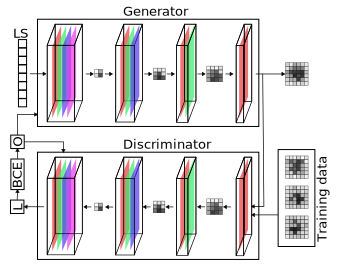
\includegraphics[width=0.6\linewidth]{images/network.png}
  \caption[]{Graphical model of our network used for generation of
    shapes. \\ \textit{Normal workflow}: A random vector from the latent space
    (\textbf{LS}) is feeded to the generator which produces a $92 \times 92$
    grayscale image of a random shape. \\ \textit{Training workflow}: The
    discriminator tries to distinguish generated images and images from the
    training set by associating an image with a label (\textbf{L}) (0 for a
    generated image, 1 for an image from the training set). Then binary cross
    entropy (\textbf{BCE}) loss is calculated and the ADAM optimizer
    (\textbf{O}) tries to minimize it by adjusting trainable parameters of the
    both networks.}
  \label{fig:network}
\end{figure*}

In this work, we train three GANs using three different sets of hand-drawn
shapes, each set consisting 100 images. Also, an additional GAN is trained using
MNIST dataset\cite{deng2012mnist}. Networks are trained by minimizing binary
cross entropy loss for the both generator and discriminator. The training is
performed in batches of 10 images (a batch of real images following a batch of
fakes) for 3000 epochs (3 for the MNIST set). To diversify our small set of real
shapes each shape is rotated by a random angle around its center or can be
randomly (with probability $1/2$) flipped along horizontal and vertical axes.

We use ADAM optimizer\cite{kingma2014adam} with learning rate $2 \cdot 10^{-4}$
and $l^2$ regularization coefficient $10^{-4}$ to minimize the loss functions
for the both networks in a GAN.

Results of work of trained generator networks can be seen in the
\cref{sec:results}.

\section{Results}
\label{sec:results}
In our work we train 4 GAN networks based on 4 different datasets (dataset's
name in gray):
\begin{itemize}
\item The MNIST dataset, \code{MNIST};
\item Shapes with convexity close to (but less than) 1, \code{mostlyconvex};
\item Shapes with convexity in the range between $0.5$ and $0.6$, \code{normal};
\item Shapes consisting of thin lines and having very low convexity, \code{thin}.
\end{itemize}

Final results, upsampled to $1000 \times 1000$ pixels using \code{convert}
utility from ImageMagick\cite{imagemagick} package are on
\cref{fig:images-gan}. Also we provide our networks made in PyTorch along with a
Jupyter notebook which explains how to use them in supplementary materials to
this paper. An archive with 4000 images generates by those networks is freely
available on Github\cite{shapes-dataset}.
\begin{figure*}[tp]
  \centering
  \subfigure[\code{MNIST}]{
    \includegraphics[width=0.3\linewidth]{images/mnist.png}}
  \subfigure[\code{mostlyconvex}]{
    \includegraphics[width=0.3\linewidth]{images/mostlyconvex.png}}
  \vskip\baselineskip
  \subfigure[\code{normal}]{
    \includegraphics[width=0.3\linewidth]{images/normal.png}}
  \subfigure[\code{thin}]{
    \includegraphics[width=0.3\linewidth]{images/thin.png}}
  \caption[]{Examples of shapes generated by 4 neural networks.}
  \label{fig:images-gan}
\end{figure*}

To quantify variety of our shapes we provide a scatter plot \cref{fig:e-r} of
our shapes in elongation-roundness ($E$-$R$) space. We also build a histogram of
distribution of the shape factor $F = (E+R)/2$ proposed by \highlight{Karsanina}
et~al.\cite{PLoS_ONE} for our dataset. In the histogram we adopt the authors'
morphology classification present in \cref{tab:morph-classes}.
\begin{table*}[!htp]
  \centering
  \begin{tabular}{|c|c|}
    \hline
    Morphology class & Shape factor \\
    \hline
    Elongated dissected & 0.2 - 0.4 \\
    \hline
    Isometric dissected & 0.4 - 0.6 \\
    \hline
    Isometric slightly dissected & 0.6 - 0.8 \\
    \hline
    Round & 0.8 - 1 \\
    \hline
  \end{tabular}
  \caption{Different morphology classes and corresponding shape factors}
  \label{tab:morph-classes}
\end{table*}

\begin{figure*}[tp]
  \centering
  \includegraphics[width=0.45\linewidth]{images/roundness-elongation.png}
  \hfill
  \includegraphics[width=0.45\linewidth]{images/shape-factor.png}
  \caption[]{\textit{Left}: Scatter plot of the shapes in elongation-roundness
    ($E$-$R$) space. \textit{Right}: histogram of distribution of the shape
    factor $F = (E+R)/2$ for the shapes in our dataset.}
  \label{fig:e-r}
\end{figure*}

\bibliography{paper}
\end{document}
